% 94-29(94쪽) — $\seg{AB}=6$, $\seg{AC}=4$, $A=60^\circ$ 인 삼각형 $\pt{ABC}$(원문 「오른쪽 그림」). 스캔 화질이 낮아 TikZ 로 다시 그림.
% 라벨은 원문 것만: $6$·$4$·$60^\circ$ 와 꼭짓점 이름. 원문의 점선 치수 보조호는 라벨 위치가 대신하므로 생략했다.
% 외접원의 반지름(답)이 읽히지 않게 외접원·눈금은 그리지 않는다.
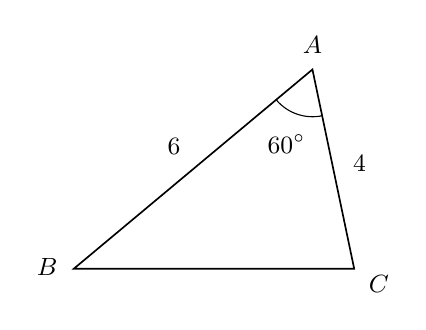
\begin{tikzpicture}[line width=0.6pt]
  \draw (0,0) -- (3.56,0) -- (3.03,2.53) -- cycle;
  \draw[line width=0.4pt] (2.570,2.145) arc (-140.1:-78.2:0.6);
  \node[font=\small] at (2.70,1.58) {$60^\circ$};
  \node[font=\small] at (1.271,1.556) {$6$};
  \node[font=\small] at (3.628,1.335) {$4$};
  \node[anchor=south, font=\small] at (3.03,2.60) {$\pt{A}$};
  \node[anchor=east, font=\small] at (-0.08,0.02) {$\pt{B}$};
  \node[anchor=north west, font=\small] at (3.62,0.04) {$\pt{C}$};
\end{tikzpicture}
